\documentclass[runningheads]{llncs}
%

% use this file to include packages and create macros

\usepackage[utf8]{inputenc}

\usepackage{subcaption}
\usepackage{framed}
\usepackage{amsfonts,amsmath}
%\usepackage{amsfonts,amssymb,amsmath,amsthm}

\usepackage{listings}
\lstset{basicstyle=\ttfamily, numbers=left, numbersep=5pt, numberstyle=\tiny, stepnumber=1, escapechar=\!, columns=fullflexible, morekeywords={true, false, a, @prefix}}

\usepackage{booktabs} % For formal tables

\usepackage{tikz, tabularx} % for drawing
\usetikzlibrary{patterns}
\usepackage{pgfplots}
\usetikzlibrary{positioning, arrows}  % use: above left of, etc
% tikz macros
\newcounter{c}
\newcounter{head}
\newcounter{tail}

\newcommand{\Symbol}[4]{
    \node at (#1,#2) [draw, circle] (#3) {#4};
}

\newcommand{\Nodeset}[5]{
    \setcounter{c}{0}
    \foreach \v in {#4} {
        \node (#1-\thec) [draw] at (#2, -{\thec/2+#3}) {$\v$};
        \setcounter{tail}{\thec}
        \stepcounter{c}
    }
    
    \ifnum \thec=0%
        \node (#1-\thec) [draw, dashed, minimum width=.45cm] at (#2, -{\thec/2+#3}) {};
        \setcounter{tail}{\thec}
        \stepcounter{c}
    \fi
    
    \stepcounter{c}
    \setcounter{head}{\thec}
    
    \foreach \v in {#5} {
        \node (#1-\thec) [draw] at (#2, -{\thec/2+#3}) {$\v$};
        \stepcounter{c}
    }

    \ifnum \thec=\thehead
        \node (#1-\thehead) [draw, dashed] at (#2, -{\thec/2+#3}) {};
    \fi
    
    \draw[->, >=stealth] (#1-\thehead) to (#1-\thetail);
}

\usepackage{hyperref} % for links
\usepackage{amsmath}

\usepackage[ruled, vlined, linesnumbered]{algorithm2e} % For algorithms
\renewcommand{\algorithmcfname}{ALGORITHM}

% math symbols
\newcommand{\ldb}{\mathopen{\lbrack\!\lbrack}}
\newcommand{\rdb}{\mathclose{\rbrack\!\rbrack}}
\newcommand{\derives}{\Rightarrow^*}
\newcommand{\T}{\mathit{traces}}
\def\bigO{\hbox{$\mathcal {O}$}}
%\newcommand{\tuple}[1]{( #1 )}
\newcommand{\set}[1]{\{ #1 \} }
\newcommand{\pr}[2]{#1 \rightarrow #2}
\newcommand{\Rule}[2]{#1 \to #2}
\newcommand{\R}[2]{\ensuremath{R(\mathit{#1},\mathit{#2}})}
\newcommand{\rules}{P}
\newcommand{\nonterminals}{N}
\newcommand{\terminals}{\ensuremath{\Sigma}}
\newcommand{\observers}{O}
\newcommand{\nil}{\textbf{nil}}
\newcommand{\ttable}{T_G}
\newcommand{\res}{\textit{res}}
\newcommand{\resm}{\res^\bullet}
\newcommand{\resu}{\res^\circ}
\newcommand{\vis}{\textit{vis}}
\newcommand{\vism}{\vis^\bullet}
\newcommand{\visu}{\vis^\circ}
\newcommand{\sta}{\textit{dscr\/}}
\newcommand{\stam}{\sta^\bullet}
\newcommand{\stau}{\sta^\circ}
\newcommand{\m}{^\bullet}
\renewcommand{\u}{^\circ}

% SPARQL commands
\newcommand{\SELECT}{\texttt{SELECT}}
\newcommand{\WHERE}{\texttt{WHERE}}
\newcommand{\AND}{\texttt{.}} % the 'AND' in SPARQL is actually a dot '.' -- ciro
\newcommand{\OPT}{\texttt{OPT}}
\newcommand{\OR}{\texttt{OR}}
\newcommand{\USING}{\texttt{USING}}
\newcommand{\FROM}{\texttt{FROM}}
\newcommand{\FILTER}{\texttt{FILTER}}
\newcommand{\var}[1]{\texttt{?#1}}
\newcommand{\inv}[1]{\overline{#1}} % 
%\newcommand{\inv}[1]{\char`\^\!#1} % SPARQL's inverse operator is '^' and it comes before the predicate

%\newcommand{\rep}[3]{#1 \ensuremath{\sim\!\! >} #2 \ensuremath{<\!\!\sim} #3}

\newcommand{\rep}[3]{\texttt{<}#1\texttt{>}#2\texttt{<}#3\texttt{>}}

% For drawing RDF graphs
\newcommand{\rdfedge}[4]{\draw [->, sloped, >=stealth, above, #4] (#1) to node {\texttt{#2}} (#3);}
\newcommand{\rdfnode}[3]{\node[draw, #3] (#1)
{\texttt{#2}};}
\newcommand{\rdfproperty}[5]{\node[minimum width=0, minimum height=0, #4 of #1] (#1-#2)
{\texttt{#3}};\rdfedge{#1}{#2}{#1-#2}{#5};}
\newcommand{\rdfloop}[3]{\path (#1) edge [loop #2,->, >=stealth, thick,red] node {#2}  (#1);}


%\newtheorem{theorem}{Theorem}
%\providecommand\definitionautorefname{Theorem}

% \newtheorem{lemma}{Lemma}
% \providecommand\definitionautorefname{Lemma}

% \newtheorem{corollary}{Corollary}
% \providecommand\definitionautorefname{Corollary}

% \newtheorem{definition}{Definition}
% \providecommand\definitionautorefname{Definition}

\newtheorem{grammar}{Grammar}
\providecommand\grammarautorefname{Grammar}

\usepackage{newfloat} % For query environment
\DeclareFloatingEnvironment[fileext=frm,placement={!ht},name=Query]{query}
% \captionsetup[query]{labelfont=bf}

\newcounter{numberInTrivlist}

\newenvironment{numtrivlist}{\begin{list}
          {\rm \arabic{numberInTrivlist})}
          {\usecounter{numberInTrivlist}
          \setlength{\leftmargin}{0pt}
          \setlength{\rightmargin}{0pt}
          \setlength{\itemindent}{12pt}
          \setlength{\listparindent}{0pt}}}
                            {\end{list}}

\newenvironment{itemizedTrivlist}{\begin{list}
          {\rm ~\hspace{2mm} $\bullet$\ } 
          {\setlength{\leftmargin}{0pt}
          \setlength{\rightmargin}{0pt}
          \setlength{\itemindent}{12pt}
          \setlength{\listparindent}{0pt}}}
                            {\end{list}}

\newcounter{inlineenum}
% \renewcommand{\theinlineenum}{\alph{inlineenum}}
\newenvironment{inlineenum}
  {\unskip\ignorespaces\setcounter{inlineenum}{0}%
   \renewcommand{\item}{\refstepcounter{inlineenum}{(\theinlineenum)~}}}
  {\ignorespacesafterend}


%article macros: rules to translation and reduction
\newcommand{\sem}[1]{[ \! [ #1 ] \! ]}
\newcommand{\guard}[1]{[ #1 ]}
\newcommand{\tuple}[1]{\langle #1 \rangle}
\newcommand{\trad}[1]{{\cal T}\sem{ #1 }}
\newcommand{\setof}[1]{\{ #1 \} }
\newcommand{\eval}[2]{\mathit{Eval}_{#1}(#2)}
\def\vertices{{\cal V}}
%\def\tr{\rhd}    % transition relation
\def\tr{\rightarrow}    % transition relation
\newcommand{\fpfrule}[2]{{{{\displaystyle #1}\over{\displaystyle #2}}}}
\newcommand{\pfrule}[2]{\begin{array}{c} #1 \\ \hline #2 \end{array}}
\newcommand{\pfruleN}[3]{\begin{array}[b]{c} #1 \\ \hline #3 \end{array} \ (#2)}
%my macros
%\newcommand{\set}[1]{\lbrace #1 \rbrace}

\newcommand{\rec}{\texttt{rec}}




% comments
\usepackage{ulem}
\normalem
\newcommand{\ourremark}[3]{\noindent{{\footnotesize\sffamily\textcolor{#2}{#3\textsuperscript{#1}}}}}
\newcommand{\mm}[1]{\ourremark{\tiny Martin}{red}{#1}}
\newcommand{\ciro}[1]{\ourremark{\tiny Ciro}{blue}{#1}}
\newcommand{\gsv}[1]{\ourremark{\tiny Semyon}{orange}{#1}}
\newcommand{\umberto}[1]{\ourremark{\tiny Umberto}{purple}{#1}}

%\hypersetup{draft}

\pgfplotsset{compat=1.14}


\usepackage{graphicx}
% Used for displaying a sample figure. If possible, figure files should
% be included in EPS format.
%
% If you use the hyperref package, please uncomment the following line
% to display URLs in blue roman font according to Springer's eBook style:
% \renewcommand\UrlFont{\color{blue}\rmfamily}

\begin{document}
%
\title{Recursive Expressions for SPARQL Property Paths}
%
%\titlerunning{Abbreviated paper title}
% If the paper title is too long for the running head, you can set
% an abbreviated paper title here
%

% \author{First Author\inst{1}\orcidID{0000-1111-2222-3333} \and
% Second Author\inst{2,3}\orcidID{1111-2222-3333-4444} \and
% Third Author\inst{3}\orcidID{2222--3333-4444-5555}}
% \institute{Princeton University, Princeton NJ 08544, USA \and
% Springer Heidelberg, Tiergartenstr. 17, 69121 Heidelberg, Germany
% \email{lncs@springer.com}\\
% \url{http://www.springer.com/gp/computer-science/lncs} \and
% ABC Institute, Rupert-Karls-University Heidelberg, Heidelberg, Germany\\
% \email{\{abc,lncs\}@uni-heidelberg.de}}

% \author{Ciro M. Medeiros\inst{1,2}
% \and
% Umberto S. Costa\inst{1}
% \and
% Semyon Grigorev\inst{3,4}
% 	%\orcid{0000-0002-7966-0698}
% \and
% Martin A. Musicante\inst{1}
% }

% \authorrunning{C. Medeiros et al.}

% \institute{Universidade Federal do Rio Grande do Norte, Natal, Brazil
% \email{cirommed@ppgsc.ufrn.br, \{umberto,mam\}@dimap.ufrn.br}
% \and
% Laboratoire d'Informatique Fondamentale d'Orléans, Orléans, France
% %		\streetaddress{Primorskiy prospekt 68-70, Building 1}
% %		\postcode{199034}
% \and
% Saint Petersburg State University, St. Petersburg, Russia
% \email{s.v.grigoriev@spbu.ru}
% %		\streetaddress{7/9 Universitetskaya nab.}
% %		\postcode{199034}
% \and
% JetBrains Research, St. Petersburg, Russia
% \email{semyon.grigorev@jetbrains.com}
% %		\streetaddress{Primorskiy prospekt 68-70, Building 1}
% %		\postcode{199034}
% }


\maketitle              % typeset the header of the contribution
%
\begin{abstract}
Regular expressions are used in SPARQL property paths to query RDF graphs.
However, regular expressions can only define the most limited class of languages, called regular languages.
Context-free languages are a wider class containing all regular languages.
There are no context-free expressions to define them, so it is necessary to write grammars.
We propose an extension of regular expressions, called recursive expressions, to support the definition of a subset of context-free languages.
The goal of our work is therefore to provide simple operators allowing the definition of languages as close as possible to context-free languages.
\keywords{Graphs \and Context-Free Path Queries \and Recursive Expressions.}
\end{abstract}
%
%
%
\section{Introduction}

%Query languages are domain-specific languages, specialized in fetching data items within a database.
%They are part of any database system, allowing the user to retrieve data by writing \textit{queries} over the database.

Several database models have been defined over the years, being \textit{relational da\-ta\-bases} the most well studied, due to their robustness concerning to scalability and data consistency.
Relational databases represent data in the form of n-ary relations (or tables), where each element is given as a tuple (or record).
%
Regardless the adopted database model, data are retrieved from such sources by using queries specified over a  domain-specific language.
SQL~\cite{sql} is extensively used as a query language in the context of relational database systems.

In recent years, \emph{graph databases} have become popular. 
This database model represents data as subject-predicate-object triples $(s, p, o)$, where $s$ and $o$ are nodes of the graph and $p$ is the label of the edge linking them.
The \emph{Resource Description Framework} (RDF) is W3C's recommendation for implementing Linked Data~\cite{w3c-rdf}.
An RDF database is a set of those triples.
%
SPARQL is a query language similar to SQL and is the standard query language for RDF databases.

A SPARQL query is defined by specifying paths inside the graph and using relational operators to construct the answer to the query.
SPARQL defines \emph{Property Paths}, which are patterns formed by edge labels of the graph (\textit{i.e.}, predicates, in RDF terminology).
Those patterns are used to link nodes that participate in the query.
SPARQL property paths are defined by means of regular expressions, thus defining regular paths inside the graph.

Regular expressions have proved to be useful for querying paths in RDF graph da\-ta\-bases~\cite{w3c2012sparql-query-lang}.
However, some papers address the problem of increasing the  expressiveness in path queries to support context-free languages.
The idea of this line of research is to be able to directly support queries such as the \textit{Same Generation Queries}~\cite{abiteboul1995foundations}.
Queries of this kind are called \textit{Context-Free Path Queries}~(CFPQs)~\cite{Hellings14}.
In general, these studies focus on the development of algorithms for the evaluation of such queries~\cite{Hellings14,Hellings2015pathresults,fred,grigorev2016ll,azimov-grigorev2017matrix,MEDEIROS2019}.


Most of the research efforts in the area are devoted to the definition of algorithms to implement CFPQs. 
However, a few of them propose syntactic constructors for query languages to support context-free path queries.
This is an important aspect of the query language \emph{pragmatics} that still needs to be fully addressed. 
We can mention three initiatives devoted to define non-regular query languages for graph databases.
The first one is an extension of the Cypher query language \footnote{\url{https://github.com/thobe/openCypher/blob/rpq/cip/1.accepted/CIP2017-02-06-Path-Patterns.adoc\#153-compared-to-context-free-languages}}, that proposes the definition of a query to contain a context-free grammar, whose non-terminal symbols are used inside the property path.
The proposal in~\cite{MEDEIROS2019} extends SPARQL in a similar way.
In~\cite{nsparql}, SPARQL is extended with \textit{Nested Regular Expressions}, an extension of Regular Expressions.

In this context, writing a context-free path query requires the knowledge of grammars and the use of a notation to represent them in a query format.
Whilst regular expressions as used in SPARQL are concise and widely known by the database community, context-free grammars are not as simple nor well known.

The main goal of our work is to investigate the use of an extension of regular expressions to define a meaningful subset of context-free languages.
We define \emph{recursive expressions} as an extension of regular expressions, in order to specify a subset of context-free languages.
We define the syntax and operational semantics of \textsf{rcfSPARQL} (restricted-context-free SPARQL), a query language that includes property paths built upon recursive expressions.
Although \textsf{rcfSPARQL} is not as expressive as languages for specifying general CFPQs, we argue that it presents a reasonable trade-off by combining the ease of specification provided by regular expressions and part of the expressiveness of context-free grammars.

\medskip
This paper is organized as follows.
Section~\ref{sec:grammars} presents notions about context-free languages and path queries in the context of graph databases. 
In section~\ref{sec:rec_exp} we propose the syntax of recursive expressions and formalize their meaning in terms of context-free grammars.  
In Section~\ref{sec:query_language} we show how recursive expressions can be used to specify \textsf{rcfSPARQL} queries.  
The operational semantics of \textsf{rcfSPARQL} is given in Section~\ref{sec:semantics}.
Finally, we conclude the paper in Section~\ref{sec:conclusions} by adding important remarks and directions for future work.


\section{Context-Free Languages and Path Queries over Data Graphs}
\label{sec:grammars}

An~\emph{alphabet} $\Sigma$ is a finite set of symbols.
A finite sequence of symbols from an alphabet $\Sigma$ is a~\emph{string}.
A set of strings forms a~\emph{language}.

Context-Free Languages can be generated by~\emph{Context-Free Grammars}, which are quadruples~$G=(N,\Sigma,P,S)$, where $\Sigma$ is an alphabet of terminals symbols (the alphabet of a language); $N$ is a finite set of non-terminal symbols; $P$ is a set of production rules of the form $\Rule{A}{\alpha}$, where $A \in N$ and  $\alpha \in (N\cup\Sigma)^*$, and $S\in N$ is the start symbol.

A \textit{Dyck Language} is a context-free language whose strings are formed by balanced parentheses.
Dyck languages are a proper subclass of context-free languages.
A Dyck language over $n$ balanced pairs may be specified by the following grammar: $S \to a_0 \ S \ b_0  \ S \mid \cdots \mid a_{n-1} \ S \ b_{n-1} \ S \mid \epsilon$ , where $(a_i,b_i)$ are terminals that specify i-th balanced pair.
This grammar is called a Dyck Grammar.


\medskip

A \textit{Graph Database} (also referred to as a \textit{Data Graph}) is a set of triples $(s,p,o)$, where $s$ is the subject, $p$ is the predicate and $o$ is called the object of the tuple.
The elements $s$ and $o$ are seen as vertices of a graph and $p$ is a label to a directed edge from $s$ to $o$.
In the context of RDF, $s$, $p$ and $o$ are URIs.

A \textit{Path} $\pi$ between nodes $x$ and $y$ over a graph database is defined as a sequence of triples $(t_0,\dots,t_k)$ such that:
\textit{(i)} the subject of $t_0$ is $x$;
\textit{(ii)} the object of $t_k$ is $y$; and
\textit{(iii)} for all $1 \leq i \leq k$, the object of $t_{i-1}$ is the subject of $t_i$.
The \textit{Trace} of a path $\pi$ is the sequence of edge labels (predicates) of $t_0,\dots,t_k$ preserving the order of the triples. 

The goal of a path query over a graph database is to identify paths inside the graph.
There exist a number of proposals to define path queries in query languages.
For instance, SPARQL defines them by using regular expressions.
Other proposals include Nested Regular Expressions~\cite{nsparql} or Context-Free Grammars
~\cite{Hellings14,Hellings2015pathresults,fred,grigorev2016ll,azimov-grigorev2017matrix,MEDEIROS2019}.

\section{Recursive Expressions}
\label{sec:rec_exp}

In this section we define \emph{recursive expressions}, which are an extension of regular expressions, supporting the definition of a subset of context-free languages.

The syntax of recursive expressions is given by:
\begin{eqnarray*}
    exp &\rightarrow& () \ |\ t\ |\ ( exp )\ |\ exp~exp\ |\ exp \text{$|$} exp\ |\ exp* \\
    &|&\rep{exp_1 \cdots exp_n}{\ exp\ }{exp'_n \cdots exp'_1}
\end{eqnarray*}

Notice that recursive expressions 
include the ternary \emph{recursion operator: } \rep{\_}{\_}{\_}.
Intuitively, the expressions $exp_i$ and $exp'_i$ define pairs of matching parenthesis.

%\gsv{Grammar extraction can be done in the same way as you describe in this paper, we just need to introduce new nonterminals for left and right subgroups. Something like this:
% \[
% \pfrule{
% \varphi(\rep{\alpha}{E}{\beta}) = \set{\Rule{S'}{\gamma}, \dots},
% \varphi(e_1) = \set{\Rule{S_1}{\gamma_1}, \dots},
% \varphi(e'_1) = \set{\Rule{S'_1}{\gamma'_1}, \dots}
% \qquad S\mbox{ is new}
% }{
% \varphi(\rep{e_1\ \alpha}{E}{\beta\ e'_1}) = \set{\Rule{S}{S_1\ S'\ S'_1}} \cup \set{\Rule{S_1}{\gamma_1}, \dots} \cup \set{\Rule{S'_1}{\gamma'_1}, \dots} \cup \set{\Rule{S'}{\gamma}, \dots}
% }
% \] 
% This way we can do your examples correct in terms of the definition.}


The language defined by a recursive expression can be inductively defined as it is usual for regular expressions:
\begin{align*}
{\cal L}( \text{()} ) = \emptyset &\qquad\qquad\qquad
{\cal L}( t ) = \set{t} \\
{\cal L}( \text{(}e\text{)} ) = {\cal L}( e ) &\qquad\qquad\qquad
{\cal L}( e_1\ e_2 ) = {\cal L}( e_1 ) \circ {\cal L}( e_2 )\\
{\cal L}( e_1\text{$|$} e_2 ) = {\cal L}( e_1 ) \cup {\cal L}( e_2 ) &\qquad\qquad\qquad
{\cal L}( e* ) = \cup_{i\in \mathbb{N}}{\cal L}( e^i )\\
{\cal L}(\rep{e_1 \cdots e_n}{e}{e'_n \cdots e'_1}) = &\bigcup_{i=1}^{n}\{\alpha^k \beta {\alpha'}^k\ | \alpha \in {\cal L}(e_i), \beta\in {\cal L}(e), \alpha' \in {\cal L}(e'_i), k \geq 0\}
\end{align*}

\begin{table}[h!]
\caption{Examples of Recursive Expressions.}\label{tab:examples}
\begin{center}
\begin{tabular}{|c|l|l|p{5.4cm}|}
\hline
\textbf{\#} & \textbf{Recursive Expression} & \textbf{Grammar} & \textbf{Language} \\
\hline
(1) & $\rep{a}{}{b}$ & $\begin{array}{l}
\Rule{S}{a\ S\ b}\\
\Rule{S}{\epsilon}
\end{array}$ & ~$a^n\ b^n$ \\ \hline
(2) & $(\rep{ab}{}{ab})^*$ & 
$\begin{array}{l}
S \to \epsilon\\
S \to S \ S_1 \\
S_1 \to a\ S_1\ b \\
S_1 \to b\ S_1\ a \\
S_1 \to \epsilon
\end{array}$
& Equal number of $a$'s and $b$'s. \\ \hline
(3) & $\rep{b}{a}{(bb)}$ & 
$\begin{array}{l}
\Rule{S}{b\ S\ b\ b}\\
\Rule{S}{a}
\end{array}$
& ~$b^n\ a\ b^{2n}$ \\ \hline
(4) & $\rep{sc\ t}{(sc\ \inv{sc})\ |\ (t\ \inv{t})}{\inv{t}\ \inv{sc}}$ & 
$\begin{array}{l}
\Rule{S}{sc\ S\ \inv{sc}}\\
\Rule{S}{t\ S\ \inv{t}}\\
\Rule{S}{sc\ \inv{sc}}\\
\Rule{S}{t\ \inv{t}}
\end{array}$
& Balanced pairs of $sc$ (RDF \textit{subClassOf}) and $t$ (RDF \textit{type}) edges~\cite{MEDEIROS2019}. \\ \hline
(5) & $\rep{sc}{}{\inv{sc}}\ \inv{sc}$ & 
$\begin{array}{l}
\Rule{S}{A\ \inv{sc}}\\
\Rule{A}{sc\ A\ \inv{sc}}\\
\Rule{A}{\epsilon}
\end{array}$
& Balanced pairs of $sc$ (subClassOf) edges with extra $\inv{sc}$~\cite{MEDEIROS2019}. \\ \hline
(6) & $\rep{a}{(b|c|d)^4}{\inv{a}}$ & 
$\begin{array}{l}
\Rule{S}{a\ S\ \inv{a}}\\
\Rule{S}{A}\\
\Rule{A}{B\ B\ B\ B}\\
\Rule{B}{b}\\
\Rule{B}{c}\\
\Rule{B}{d}
\end{array}$
& $a^n\ (b | c | d)^4\ (\inv{a})^n$ (see~\cite{jochemkuijpers}); the superscript $^4$ indicates 4 repetitions. \\ \hline
(7) & $a\rep{a}{(\rep{b}{}{c})}{d}d$ & 
$\begin{array}{l}
\Rule{S}{a\ A\ d}\\
\Rule{A}{a\ A\ d}\\
\Rule{A}{B}\\
\Rule{B}{b\ B\ c}\\
\Rule{B}{\epsilon}
\end{array}$
& ~$a\ a^n b^m c^m d^n\ d$ (see~\cite{jochemkuijpers}). \\ \hline
(8) & $\rep{(\rep{a}{b}{c})}
{d}
{(\rep{e}{}{f})}$ & $\begin{array}{l}
    \Rule{S}{A\ S\ B} \\
    \Rule{S}{d}\\
    \Rule{A}{a\ A\ c} \\
    \Rule{A}{b}\\
    \Rule{B}{e\ B\ f} \\
    \Rule{B}{\epsilon}
\end{array}$
& 
~$(a^n\ b\ c^n)^k\ d\ (e^m\ f^m)^k$
\\ 
\hline
\end{tabular}
\end{center}
\end{table}




Recursive expressions allow us to define a number of relevant context-free languages, including the ones found in~\cite{jochemkuijpers,MEDEIROS2019}. 
In Table~\ref{tab:examples} we show some examples of recursive expressions, equivalent context-free grammars and their languages.
We represent a grammar by its set of production rules.
In order to simplify the notation, we consider that the first non-terminal symbol appearing in a set of rules is the start symbol.
The notation $\inv{p}$ inverts the orientation of an edge, that is, if the tuple $(s,p,o)$ is in the database, so is $(o,\inv{p},s)$.
It is normally implemented by explicitly adding those edges to the database.

The examples put in evidence two characteristics of recursive expressions: conciseness and legibility.
These characteristics  may improve the pragmatics of a query language.

Notice that most of these examples are subsets of Dyck languages (in the sense that they define a language of balanced parentheses).
In this way, we can see that recursive expressions describe a subset of the class of Dyck languages.
Notice that the languages described by the recursive expressions~(2) and~(8) are not Dyck languages.
On the other hand, there are context-free languages that cannot be expressed by recursive expressions.


\subsection{Obtaining a Grammar From a Recursive Expression}
\label{sec:transforming}

Let us now define how a grammar can be obtained from a given recursive expression.
In the following rules, we inductively define the function $\varphi$, taking a recursive expression and producing a context-free grammar $G$, generating the same language.

The grammars corresponding to the recursive expressions () and $a$  generate, respectively, the empty language and the language $\set{a}$:
\[
\pfrule{
S\mbox{ is new}
}{
\varphi(\epsilon) = \set{\Rule{S}{\epsilon}}
}
\]

\[
\pfrule{
a\mbox{ is a terminal symbol}, \qquad S\mbox{ is new}
}{
\varphi(a) = \set{\Rule{S}{a}}
}
\]

The recursive expression $(E)$ can be associated with a grammar that generates the same language as $E$:
\[
\pfrule{
\varphi(E_1) = \set{\Rule{S_1}{\alpha}, \dots}, \qquad S\mbox{ is new}
}{
\varphi(\ (E_1)\ ) = \set{\Rule{S}{S_1}} \cup \varphi(E_1)
}
\]
The grammars associated to sequential, alternative and Kleene star operators are computationally defined by adding a new start symbol and rules for concatenation, choice and repetition of strings:
\[
\pfrule{
\varphi(E_1) = \set{\Rule{S_1}{\alpha}, \dots}, \qquad \varphi(E_2) = \set{\Rule{S_2}{\beta}, \dots},\qquad S\mbox{ is new}
}{
\varphi(E_1\ E_2) = \set{\Rule{S}{S_1\ S_2}} \cup \varphi(E_1) \cup \varphi(E_2)
}
\]

\[
\pfrule{
\varphi(E_1) = \set{\Rule{S_1}{\alpha}, \dots}, \qquad \varphi(E_2) = \set{\Rule{S_2}{\beta}, \dots},\qquad S\mbox{ is new}
}{
\varphi(E_1\ | E_2) = \set{\Rule{S}{S_1}, \Rule{S}{S_2}} \cup \varphi(E_1) \cup \varphi(E_2)
}
\]



\[
\pfrule{
\varphi(E_1) = \set{\Rule{S_1}{\alpha}, \dots}, \qquad S\mbox{ is new}
}{
\varphi( E_1^*) = \set{\Rule{S}{S_1\ S}, \Rule{S}{\epsilon}} \cup \varphi(E_1)
}
\]


% \mm{This next rule allows just terminals as brackets.}
% \[
% \pfrule{
% \varphi(E) = \set{\Rule{S'}{\gamma}, \dots},
% \qquad S\mbox{ is new},
% \qquad R = \set{\Rule{S}{a_i\ S'\ b_i}\ |\ i\in\set{1,\dots,n}}
% }{
% \varphi(\rep{a_1\dots a_n}{E}{b_n\dots b_1}) = R \cup \varphi(E)
% }
% \]


The rule for obtaining a grammar that generates the language for the expression $\rep{E_1 \dots E_n}{\ E\ }{E'_n\dots E'_1}$ proceeds by:
\textit{(i)} generating context-free grammars for all the sub-expressions;
\textit{(ii)} building the set $R$, formed by the union of all these grammars and the set of rules $\set{\Rule{S}{S_i\ S''\ S'_i}\ |\ i\in\set{1,\dots,n}}$.
The rules in this set define the matching of strings generated by each pair of expressions $E_i$ and $E'_i$:
\[
\pfrule{ 
\varphi(E_i) = \set{\Rule{S_i}{\alpha_i}, \dots}\quad \mbox{ for all } i\in\set{1,\dots,n},\\
\varphi(E'_i) = \set{\Rule{S'_i}{\alpha'_i}, \dots}\quad \mbox{ for all } i\in\set{1,\dots,n},\\
\qquad \varphi(E) = \set{\Rule{S''}{\beta}, \dots}, \qquad S\mbox{ is new}\\
R = \varphi(E_1) \cup \dots \cup \varphi(E_n) \cup \varphi(E'_1) \cup \dots \cup \varphi(E_n)
}{
\varphi(\rep{E_1 \dots E_n}{\ E\ }{E'_n\dots E'_1}) = \set{\Rule{S}{S''}} \cup \set{\Rule{S}{ S_i S\ S_i'}\ |\ i\in\set{1,\dots,n}} \cup R
}
\]

The grammar defined by a recursive expression will be used in the next sections to define the semantics of \textsf{rcfSPARQL}, a query language inspired by SPARQL.




\section{A Query Language Containing Recursive Expressions}
\label{sec:query_language}

In this section we present \textsf{rcfSPARQL}, a query language that uses recursive expressions to build non-regular property paths.

The syntax of \textsf{rcfSPARQL} adapts \textsf{cfSPARQL} by using recursive expressions to define property paths (instead of non-terminal symbols used in \textsf{cfSPARQL}).
This eliminates the need to define a context-free grammar in the query.
First, we define the syntax of triple and graph patterns and then we will use them to build queries in \textsf{rcfSPARQL}.

\begin{definition}[Restricted Context-Free Triple Pattern]
A \textit{restricted con\-text-free triple pattern} ${\cal T}$ is a tuple of the form $(qs, qp, qo)$, where $qs, qo$ are literals or variables and $qp$ is a literal, variable or recursive expression over literals.
\hfill$\Box$
\end{definition}

The next definition presents Restricted Context-Free Graph Patterns, used to combine restricted context-free triple patterns.
Restricted graph patterns correspond to SPARQL operators, being the basis for building queries, by handling and combining sets of tuples.

\begin{definition}[Restricted Context-Free Graph Pattern]
A \textit{restricted con\-text-free graph pattern} ${\cal P}$ is a graph pattern built from restricted context-free triple patterns and SPARQL operations, in accordance with the following grammar:
\begin{align*} 
{\cal P} &\rightarrow
  \begin{array}[t]{l}
  {\cal T} \ \mid\  {\cal P}\  \texttt{.}\ {\cal P} \ \mid\    {\cal P}\ \texttt{OPT}\ {\cal P} \  \mid\  {\cal P}\ \texttt{UNION}\  {\cal P}\ \mid\  {\cal P}\   \texttt{FILTER}\ {\cal E}
  \end{array} \\
{\cal E} &\rightarrow
  \begin{array}[t]{l}
  \textit{bound}(?x)
  \ |\ ?x\ \textit{op}\ l
  \ |\ ?x\ \textit{op}\ ?y
  \ |\ \neg {\cal E}
  \ |\ {\cal E} \wedge {\cal E}
  \ |\ {\cal E} \vee {\cal E}
\end{array}
\end{align*}
where $?x$, $?y$ are variables, \textit{l} is a literal, $\textit{op} \in \set{<, \leq, >, \geq, =, \neq}$, and ${\cal T}$ is a restricted context-free triple pattern. 
\hfill$\Box$
\end{definition}

We define a \emph{Restricted Context-Free SPARQL} (\textsf{rcfSPARQL}) query as follows:


\begin{definition}[Restricted Context-Free Graph Query]
Given an RDF data graph $D$ and a list of variable identifiers $?x_1, \dots, ?x_n$, a restricted context-free graph query ${\cal Q}$ is defined as:
$$ \qquad \qquad \qquad
{\cal Q} \rightarrow \ \texttt{SELECT}\ ?x_1, \dots, ?x_n\ \texttt{FROM}\ D\ \texttt{WHERE}\ {\cal P}
$$
where ${\cal P}$ is a restricted context-free graph pattern.
\hfill$\Box$
\end{definition}


The following example (adapted from~\cite{MEDEIROS201975}) illustrates the use of recursive expressions in an \textsl{rcfSPARCL} query. 

\begin{example} \label{ex}
Let $D$ be the database in Figure~\ref{fig:ex-employees}.
It contains information about a company's employees.
We rewrite the query in~\cite{MEDEIROS2019} that selects the employees having have the same job, but different salaries.
The query is written in \textsf{rcfSPARQL} as:
\begin{lstlisting}
SELECT ?job, ?emp1, ?sal1, ?emp2, ?sal2 !\label{l:select2}!
FROM D
WHERE {
   ?emp1 !$\rep{\mathtt{boss}}{}{\mathtt{\inv{boss}}}$! ?emp2 . !\label{l:rec-pattern}!
   ?emp1 job ?job . !\label{l:emp1-job-pattern2}!
   ?emp2 job ?job . !\label{l:emp2-job-pattern2}!
   ?emp1 salary ?sal1 . !\label{l:sal1-pattern2}!
   ?emp2 salary ?sal2 . !\label{l:sal2-pattern2}!
   FILTER (?sal1 > ?sal2) !\label{l:filter-pattern2}!
!\}!
    \end{lstlisting}

\begin{figure}[htb]
    \centering
    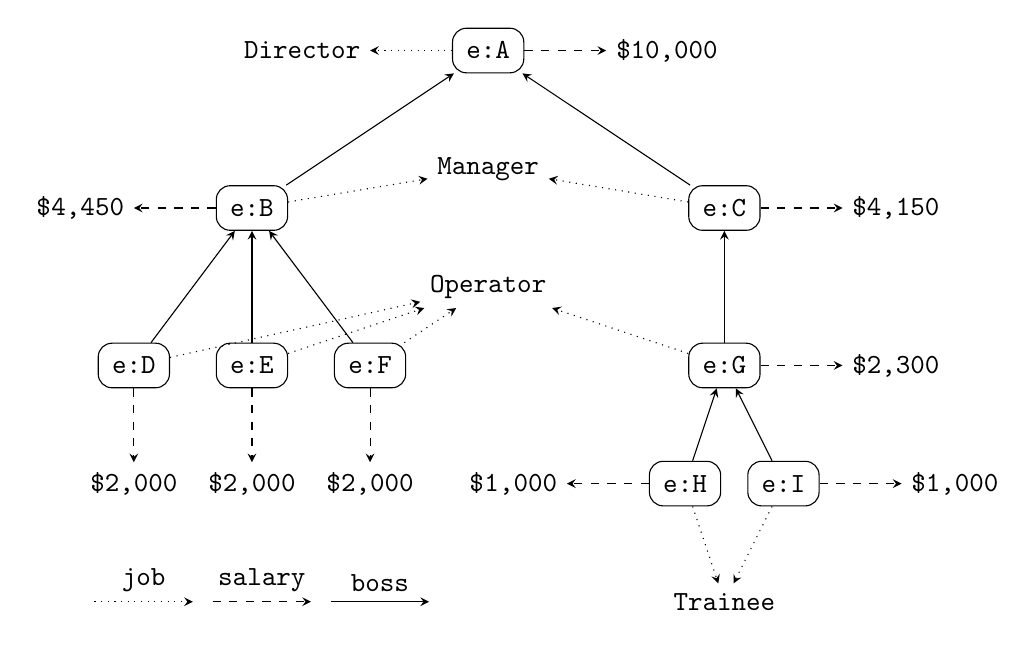
\begin{tikzpicture}[level/.style={sibling distance=20mm/#1}]

\node[inner sep=5pt, draw, rectangle, rounded corners=5pt] at (0,0) (a) {\texttt{e:A}};
\node[inner sep=5pt, draw, rectangle, rounded corners=5pt] at (-3,-2) (b) {\texttt{e:B}};
\node[inner sep=5pt, draw, rectangle, rounded corners=5pt] at (3,-2) (c) {\texttt{e:C}};
\node[inner sep=5pt, draw, rectangle, rounded corners=5pt] at (-4.5,-4) (d) {\texttt{e:D}};
\node[inner sep=5pt, draw, rectangle, rounded corners=5pt] at (-3,-4) (e) {\texttt{e:E}};
\node[inner sep=5pt, draw, rectangle, rounded corners=5pt] at (-1.5,-4) (f) {\texttt{e:F}};
\node[inner sep=5pt, draw, rectangle, rounded corners=5pt] at (3,-4) (g) {\texttt{e:G}};
\node[inner sep=5pt, draw, rectangle, rounded corners=5pt] at (2.5,-5.5) (h) {\texttt{e:H}};
\node[inner sep=5pt, draw, rectangle, rounded corners=5pt] at (3.75,-5.5) (i) {\texttt{e:I}};

\draw [->, sloped, >=stealth] (b) to node [auto] {} (a);
\draw [->, sloped, >=stealth] (c) to node [auto] {} (a);
\draw [->, sloped, >=stealth] (d) to node [auto] {} (b);
\draw [->, sloped, >=stealth] (e) to node [auto] {} (b);
\draw [->, sloped, >=stealth] (f) to node [auto] {} (b);
\draw [->, sloped, >=stealth] (g) to node [auto] {} (c);
\draw [->, sloped, >=stealth] (h) to node [auto] {} (g);
\draw [->, sloped, >=stealth] (i) to node [auto] {} (g);

\node[anchor=west] at (1.5,0) (sa) {\texttt{\$10,000}};
\node[anchor=east] at (-4.5,-2) (sb) {\texttt{\$4,450}};
\node[anchor=west] at (4.5,-2) (sc) {\texttt{\$4,150}};
\node at (-4.5,-5.5) (sd) {\texttt{\$2,000}};
\node at (-3,-5.5) (se) {\texttt{\$2,000}};
\node at (-1.5,-5.5) (sf) {\texttt{\$2,000}};
\node[anchor=west] at (4.5,-4) (sg) {\texttt{\$2,300}};
\node[anchor=east] at (1,-5.5) (sh) {\texttt{\$1,000}};
\node[anchor=west] at (5.25,-5.5) (si) {\texttt{\$1,000}};

\draw [->, >=stealth, dashed] (a) to node [auto] {} (sa);
\draw [->, >=stealth, dashed] (b) to node [auto] {} (sb);
\draw [->, >=stealth, dashed] (c) to node [auto] {} (sc);
\draw [->, >=stealth, dashed] (d) to node [auto] {} (sd);
\draw [->, >=stealth, dashed] (e) to node [auto] {} (se);
\draw [->, >=stealth, dashed] (f) to node [auto] {} (sf);
\draw [->, >=stealth, dashed] (g) to node [auto] {} (sg);
\draw [->, >=stealth, dashed] (h) to node [auto] {} (sh);
\draw [->, >=stealth, dashed] (i) to node [auto] {} (si);

\node[anchor=east] at (-1.5,0) (ja) {\texttt{Director}};
\node at (0,-1.5) (jbc) {\texttt{Manager}};
% \node[anchor=west] at (4,-1.5) (jc) {\texttt{Manager}};
\node at (0,-3) (jdefg) {\texttt{Operator}};
% \node at (-2.5,-5.5) (je) {\texttt{Operator}};
% \node at (-1,-5.5) (jf) {\texttt{Operator}};
% \node[anchor=west] at (4,-3.5) (jg) {\texttt{Operator}};
\node at (3,-7) (jhi) {\texttt{Trainee}};
% \node[anchor=west] at (4.75,-5.5) (ji) {\texttt{Trainee}};

\draw [->, >=stealth, dotted] (a) to node [auto] {} (ja);
\draw [->, >=stealth, dotted] (b) to node [auto] {} (jbc);
\draw [->, >=stealth, dotted] (c) to node [auto] {} (jbc);
\draw [->, >=stealth, dotted] (d) to node [auto] {} (jdefg);
\draw [->, >=stealth, dotted] (e) to node [auto] {} (jdefg);
\draw [->, >=stealth, dotted] (f) to node [auto] {} (jdefg);
\draw [->, >=stealth, dotted] (g) to node [auto] {} (jdefg);
\draw [->, >=stealth, dotted] (h) to node [auto] {} (jhi);
\draw [->, >=stealth, dotted] (i) to node [auto] {} (jhi);

\draw [->, >=stealth, dotted] (-5,-7) to node [auto] {\texttt{job}} (-3.75,-7);
\draw [->, >=stealth, dashed] (-3.5,-7) to node [auto] {\texttt{salary}} (-2.25,-7);
\draw [->, sloped, >=stealth] (-2,-7) to node [auto] {\texttt{boss}} (-0.75,-7);

\end{tikzpicture}
\caption{Example of hierarchy database $D$~\cite{MEDEIROS2019}.}
\label{fig:ex-employees}
\end{figure}
This query defines a relation formed by 5-tuples.
The variables at line (1) define the attributes of this relation.
The property path at line (4) defines a path between pairs of employees (\texttt{?emp1} and \texttt{?emp2}).
Notice that this path uses a recursive expression to look for paths between employees at the same level of the hierarchy.
These paths will be formed by nested \texttt{boss} and $\mathtt{\inv{boss}}$ edges.

Lines (5-8) of the query looks, respectively, for the jobs and salaries of each pair of employees identified in line (4).
Notice that there is just one variable \texttt{?job}, denoting that both employees have the same position in the company.
Line (9) filters the pairs of employees that have the same job but different salaries.
\hfill$\Box$
\end{example}

\section{Answering \textsf{rcfSPARQL} Queries}
\label{sec:semantics}

This section presents a formal semantics for \textsf{rcfSPARQL}.
We adapt the operational semantics given in~\cite{MEDEIROS2019} to consider restricted context-free graph patterns.

Similarly to other declarative query languages such as SPARQL~\cite{SPARQL} and SQL~\cite{sql}, queries in \textsf{rcfSPARQL} rely upon the notion of \emph{relations}.
We use the same RDF data representation as in~\cite{MEDEIROS2019}.
This representation defines a three-level tree for each relational table.
In this tree, the root node represents the whole table.
On the second level there is a node for each line of the table (these nodes are linked to the root by \rec-labeled edges).
The information stored in the table appears on the leaves.
Each value is linked to its corresponding record node by using edges labeled according to a column of the table.




Let us now define the function $\varphi({\cal P})$ as an extension of the function $\varphi$ for recursive expressions.
The function $\varphi({\cal P})$ takes a restricted context-free graph pattern and returns a new context-free graph pattern, similar to ${\cal P}$, but replacing each recursive expression for one (literal) non-terminal symbol of $G$, generating the same language as the recursive expression.
The function $\varphi$ over patterns is defined as follows:
\[
\pfrule{
gp\mbox{ is a terminal symbol or query variable}%\ciro{\sout{\textit{not} a recursive expression}}
}{
\varphi((gs, gp, go)) = (\emptyset, (gs, gp, go))
}
\]

\[
\pfrule{
E\mbox{ is a recursive expression}, \qquad
\set{\Rule{S}{\alpha}, \dots} = \varphi(E)
}{
\varphi((gs, E, go)) = (\varphi(E), (gs, S, go))
}
\]

\[
\pfrule{
\oplus \in \set{\texttt{AND}, \texttt{OPT}, \texttt{UNION}}, \qquad
(G_1, {\cal P}'_1) = \varphi({\cal P}_1), \qquad
(G_2, {\cal P}'_2) = \varphi({\cal P}_2)
}{
\varphi({\cal P}_1 \oplus {\cal P}_2) = ( G_1 \cup G_2, {\cal P}'_1 \oplus {\cal P}'_2)
}
\]

\[
\pfrule{
(G, {\cal P}') = \varphi({\cal P})
}{
\varphi({\cal P}\   \texttt{FILTER}\ {\cal E}) = ( G, {\cal P}'\ \texttt{FILTER}\ {\cal E})
}
\]

The operational semantics for \textsf{rcfSPARQL} is similar to cfSPARQL defined in~\cite{MEDEIROS2019} and is not reproduced here due to lack of space.
The semantic rules in~\cite{MEDEIROS2019} build an RDF graph tree containing one record for each solution of the query.

The only difference is on query evaluation, whose semantics for \textsf{rcfSPARQL} we present below.
The query to be evaluated is given in double brackets.
In order to answer a restricted context-free path query, our method proceeds in a similar manner as described in~\cite{MEDEIROS2019}. 
We have included a step to obtain a grammar $G$ from the restricted context-free pattern ${\cal P}$.
Also, we have removed steps specific to the algorithm presented in~\cite{MEDEIROS2019}, such as the construction of the predictive parsing table $\ttable$.
These steps are described as follows:
%\begin{figure}%[t]
\[
\pfrule{
(G, {\cal P}') = \varphi({\cal P}) \qquad
H = \set{(a, N)\ |\ a \in \textit{Nodes}(D), N\ is\ a\ \textit{nonterminal}\ \textit{of}\ G}
\\
%\ttable = \textit{LLParserTable}(G) \\
D_1 = \textsf{eval}(G, D, H)
\qquad
D_2 = D \cup D_1
\qquad
(r, D_3) = \sem{{\cal P}'}_{D_2}
\\
\textit{Answer} = \set{(a_1,\dots,a_n)\ |\ (r, \rec, o), 
                                     (o, \mathtt{?x}_1, a_1), \dots, 
                                     (o, \mathtt{?x}_n, a_n) \in D_3}
}{\sem{\texttt{SELECT}\ \mathtt{?x}_1, \dots, \mathtt{?x}_n\ \texttt{FROM}\ D\ \texttt{WHERE}\ {\cal P}} = \textit{Answer}}
\]
%     \caption{RDF Semantics for \textsf{rcfSPARQL} Queries}
%     \label{fig:cfqueriesSemantics}
% \end{figure}

The semantics presented in the rule above %Figure~\ref{fig:cfqueriesSemantics} 
is explained next.
We will use Example~\ref{ex} to show the application of each step in obtaining the answer to the query.
These steps are as follows:
\begin{enumerate}
    \item \textit{Obtaining a context-free grammar:} A grammar $G$ is built from the restricted context-free graph pattern ${\cal P}$ by using the algorithm provided in Section~\ref{sec:transforming}.
    A new pattern ${\cal P}'$ is also built, to replace the recursive expressions in ${\cal P}$ for non-terminal symbols of the grammar $G$ describing the same language.
    
    \smallskip
    \framebox{\begin{minipage}[t]{0.93\textwidth}\textsl{
    For the query of Example~\ref{ex}, the recursive expression $\mathtt{\rep{boss}{}{\inv{boss}}}$ (line~\ref{l:rec-pattern}) is used to define the pair formed by the grammar $\set{\Rule{S}{boss\ \inv{boss}}, \Rule{S}{\epsilon}}$ and the pattern $(\text{\texttt{?emp1}}, S, \text{\texttt{?emp2}})$.}
    \end{minipage}}
    \smallskip

    \item \textit{Building a set of pairs:} The set $H$ is built to contain all pairs formed by nodes of the RDF data graph and non-terminal symbols of $G$;
    
    \smallskip
    \framebox{\begin{minipage}[t]{0.93\textwidth}\textsl{
        In Example~\ref{ex}, $H=\{$(e:A,S), (e:B,S), (e:C,S), (e:D,S), (e:E,S), (e:F,S), (e:G,S), (e:H,S), (e:I,S)\}.
        }
        \end{minipage}
    }
    \smallskip
    
    
    \item \textit{Decoration of the data graph:} In this step we use a context-free path query engine to process the set of pairs $H$.
    The function $eval$ may be replaced by any CFPQ evaluation engine used to create new edges in $D$ (proposals may be found in~\cite{Hellings14,Hellings2015pathresults,azimov-grigorev2017matrix,MEDEIROS2019}).
    Each new edge  $(x, S, y)$ indicates that there is an $S$-generated path between $x$ and $y$.
    
    \smallskip
    \framebox{\begin{minipage}[t]{0.93\textwidth}\textsl{
        The decorated graph from Example~\ref{ex} can be seen in Figure~\ref{fig:decorated}, where double ended edges mean two edges in the forward and backward senses.
        }
    \end{minipage}
    }
    \begin{figure}[h!]
        \centering
        \input{ex-decorated}
        \caption{Decorated graph.}
        \label{fig:decorated}
    \end{figure}
    \smallskip
    
    \item \textit{Query answering over the decorated graph:} In this step, the pattern ${\cal P}'$ is used to build the answer to the query over the decorated data graph $D_2$ (built in the previous step).
    The RDF graph $D_3$ is built using the semantics of the pattern ${\cal P}'$, as defined in~\cite{MEDEIROS2019}.
    
    \smallskip
    \framebox{\begin{minipage}[t]{0.93\textwidth}\textsl{
        The graph $D_3$ for our Example~\ref{ex} is depicted in Figure~\ref{fig:ex-tableRDF} (right-hand side).
        }
    \end{minipage}
    }    
    \begin{figure}[h]
        \centering
        \begin{tabular}{|c|c|c|c|c|} \hline
\textbf{?job} & \textbf{?emp1} & \textbf{?sal1} & \textbf{?emp2} & \textbf{?sal2} \\ \hline
Manager  & e:B & \$4450 & e:C & \$4150\\ \hline
Operator & e:G & \$2300 & e:D & \$2000 \\ \hline
Operator & e:G & \$2300 & e:E & \$2000 \\ \hline
Operator & e:G & \$2300 & e:F & \$2000 \\ \hline
\end{tabular}
\qquad
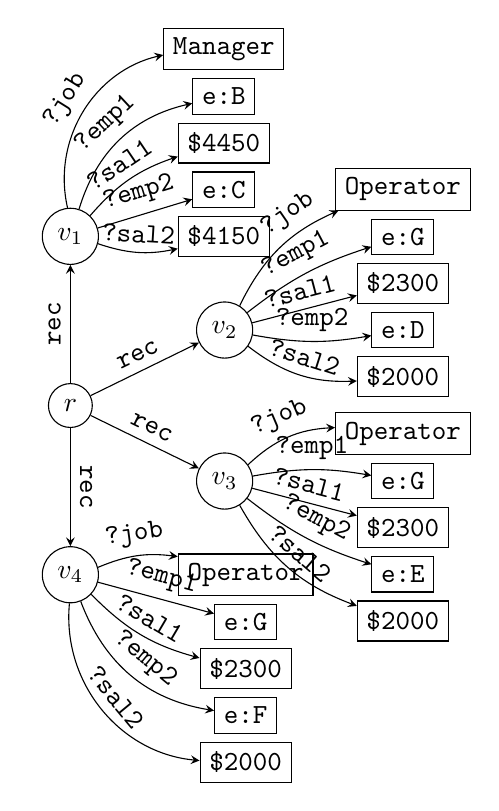
\begin{tikzpicture}[level/.style={sibling distance=8mm/#1}, baseline=(current bounding box.center)] % baseline centralizes the table vertically

\rdfnode{r}{$r$}{circle};
\rdfnode{v1}{$v_1$}{above = 1.5 of r, circle};
\rdfnode{v2}{$v_2$}{above right = 0.5 and 1.5 of r, circle};
\rdfnode{v3}{$v_3$}{below right = 0.5 and 1.5 of r, circle};
\rdfnode{v4}{$v_4$}{below = 1.5 of r, circle};

\rdfnode{sal2v1}{\$4150}{right= of v1};
\rdfnode{emp2v1}{e:C}{above= 0.1 of sal2v1};
\rdfnode{sal1v1}{\$4450}{above= 0.1 of emp2v1};
\rdfnode{emp1v1}{e:B}{above= 0.1 of sal1v1};
\rdfnode{jobv1}{Manager}{above= 0.1 of emp1v1};
\rdfedge{v1}{\textbf{?job}}{jobv1}{bend left = 45};
\rdfedge{v1}{\textbf{?emp1}}{emp1v1}{, bend left = 30};
\rdfedge{v1}{\textbf{?sal1}}{sal1v1}{bend left = 15};
\rdfedge{v1}{\textbf{?emp2}}{emp2v1}{};
\rdfedge{v1}{\textbf{?sal2}}{sal2v1}{bend right=15};


\rdfnode{emp2v2}{e:D}{right= 1.5 of v2};
\rdfnode{sal1v2}{\$2300}{above= 0.1 of emp2v2};
\rdfnode{emp1v2}{e:G}{above= 0.1 of sal1v2};
\rdfnode{jobv2}{Operator}{above= 0.1 of emp1v2};
\rdfnode{sal2v2}{\$2000}{below= 0.1 of emp2v2};
\rdfedge{v2}{\textbf{?job}}{jobv2}{pos=.7, bend left = 20};
\rdfedge{v2}{\textbf{?emp1}}{emp1v2}{bend left = 10};
\rdfedge{v2}{\textbf{?sal1}}{sal1v2}{};
\rdfedge{v2}{\textbf{?emp2}}{emp2v2}{bend right =10};
\rdfedge{v2}{\textbf{?sal2}}{sal2v2}{bend right =20};


\rdfnode{emp1v3}{e:G}{right= 1.5 of v3};
\rdfnode{jobv3}{Operator}{above= 0.1 of emp1v3};
\rdfnode{sal1v3}{\$2300}{below= 0.1 of emp1v3};
\rdfnode{emp2v3}{e:E}{below= 0.1 of sal1v3};
\rdfnode{sal2v3}{\$2000}{below= 0.1 of emp2v3};
\rdfedge{v3}{\textbf{?job}}{jobv3}{bend left = 20};
\rdfedge{v3}{\textbf{?emp1}}{emp1v3}{bend left = 10};
\rdfedge{v3}{\textbf{?sal1}}{sal1v3}{};
\rdfedge{v3}{\textbf{?emp2}}{emp2v3}{bend right =10};
\rdfedge{v3}{\textbf{?sal2}}{sal2v3}{bend right =20};


\rdfnode{jobv4}{Operator}{right= of v4};
\rdfnode{emp1v4}{e:G}{below= 0.1 of jobv4};
\rdfnode{sal1v4}{\$2300}{below= 0.1 of emp1v4};
\rdfnode{emp2v4}{e:F}{below= 0.1 of sal1v4};
\rdfnode{sal2v4}{\$2000}{below= 0.1 of emp2v4};
\rdfedge{v4}{\textbf{?job}}{jobv4}{bend left=15};
\rdfedge{v4}{\textbf{?emp1}}{emp1v4}{};
\rdfedge{v4}{\textbf{?sal1}}{sal1v4}{bend right = 15};
\rdfedge{v4}{\textbf{?emp2}}{emp2v4}{bend right =30};
\rdfedge{v4}{\textbf{?sal2}}{sal2v4}{bend right =45};


\rdfedge{r}{\rec}{v1}{};
\rdfedge{r}{\rec}{v2}{};
\rdfedge{r}{\rec}{v3}{};
\rdfedge{r}{\rec}{v4}{};
\end{tikzpicture}
        \caption{Tabular and RDF representations~\cite{MEDEIROS2019} of the answer for the query from Example~\ref{ex}.}
        \label{fig:ex-tableRDF}
    \end{figure}
    \smallskip
    
    \item \textit{Selection of the graph nodes that answer the query:} The set \emph{Answer} is formed by the leaves of the RDF graph $D_3$, organized as tuples that correspond to each record, and ordered as required by the query.
    
    \smallskip
    \framebox{\begin{minipage}[t]{0.93\textwidth}\textsl{
        In Example~\ref{ex}, $Answer=\{$(Manager, e:B, \$4450, e:C, \$4150), 
(Operator, e:G, \$2300, e:D, \$2000),
(Operator, e:G, \$2300, e:E, \$2000),
(Operator, e:G, \$2300, e:F, \$2000)\}.
See Figure~\ref{fig:ex-tableRDF} (left-hand side).
        }
        \end{minipage}
    }
    \smallskip
\end{enumerate}




\section{Conclusions and Future Work}
\label{sec:conclusions}

In this paper we presented \textsf{rcfSPARQL}, a language for the specification of a  subset of CFPQs over graph databases in RDF. 
The proposed language is built around recursive expressions, which extends regular expressions in order to encompass 
a meaningful subset of  context-free languages while keeping the specification of queries easy and concise.
Both the syntax and semantics of \textsf{rcfSPARQL} is provided, as well as a running example. 

In order to implement \textsf{rcfSPARQL}, it suffices to extend the syntax of SPARQL to include the new operators and to make use of some CFPQ evaluation algorithm.
Many algorithms for the evaluation of CFPQ  are available in the literature. 
Open-source SPARQL engines may serve as a base for such an implementation.

For simplicity, we have not included convenient operators like `+' or `?' present in regular expressions nor have we defined similar versions of them for our recursive operators.
Although they can be considered syntactic sugar, these operators make expressions more concise, and therefore improve readability.

Recursive expressions are user-friendlier than context-free grammars for writing queries. However, we know that context-free grammars are more expressive than recursive expressions. 
Thus, it is relevant to formalize how recursive expressions and  context-free grammars compare in terms of expressiveness.
This is a topic of future work.




% \section{Acknowledgements} 
% This work is partly supported by INES grant CNPq/465614/2014-0 (Brazil) and Coordena\c c\~ ao de Aperfei\c coamento de Pessoal de N\'\i vel Superior - Brazil (CAPES) - Finance Code 001.



% ---- Bibliography ----
\bibliographystyle{splncs04}
\bibliography{bibliography}
%
\end{document}
